\documentclass[a5paper,10pt]{article}
\usepackage[portuguese]{babel}
%\usepackage[latin1]{inputenc}
\usepackage[utf8]{inputenc}
\usepackage[T1]{fontenc}
\usepackage{graphicx}
\usepackage[pdftex,plainpages=false,pdfpagelabels,
pagebackref,colorlinks=true,citecolor=blue,
linkcolor=black,urlcolor=blue,filecolor=blue,
bookmarksopen=true]{hyperref}
\usepackage{amsmath,amsfonts,mathrsfs,amssymb,enumitem}
\usepackage{multicol,fancyhdr,makeidx,sectsty}
\usepackage[papersize={13.3cm,20.9cm},left=1cm,
right=1cm,top=2cm,bottom=2cm]{geometry}
\usepackage{mdframed,xcolor,fourier-orns}
%\usepackage{physics}
%5.25in,8.26in


%%%%%%%%%%%%%%%%%%%%% Box Reflita %%%%%%%%%%%%%%%%%%%%%%%%%%%%%%%%%%
\newmdenv[shadow=false, shadowsize=2pt, linewidth=2pt,
frametitlerule=true, roundcorner=20pt,]{reflita}

%%%%%%%%%%%%%%%% comando regua %%%%%%%%%%%%%%%%%%%%%%%%%%%%%%%%%%%%%
\newcommand{\HRule}[1]{\rule{\linewidth}{#1}}

%%%%%%%%%%%%%%%%%%%%%%%%%%%%%%%%%%%%%%%%%%%%%%%%%%%%%%%%%%%%%%%%%%%%%
%Atalhos para notação de conjuntos
\newcommand{\cqd}{{{\hfill $\rule{2.5mm}{2.5mm}$}}\vspace{1cm}\\}
\newcommand{\sen}{\mathrm{sen}}
\newcommand{\ds}{\displaystyle}
\newcommand{\R}{\mathbb{R}}
\newcommand{\C}{\mathbb{C}}
\newcommand{\N}{\mathbb{N}}
\newcommand{\Z}{\mathbb{Z}}
\newcommand{\Q}{\mathbb{Q}}
\newcommand{\I}{\mathbb{I}}

%%%%%%%%%%%%%%%%%%%%%%%%%%%%%%%%%%%%%%%%%%%%%%%%%%%%%%%%%%%%%%%%%%%%%
%Comandos Atalhos para operações matemáticas
\newcommand{\deli}[2]{\ensuremath\frac{\partial#1}{\partial#2}}
\newcommand{\deri}[2]{\ensuremath\frac{d#1}{d#2}}
\newcommand{\nt}[4]{\ensuremath{ \int_{#1}^{#2} #3 \, \mbox{d}#4}}

%%%%%%%%%%%%%%%%%%%%%%%%%%%%%%%%%%%%%%%%%%%%%%%%%%%%%%%%%%%%%%%%%%%%%
%Atalhos para notações matemáticas, funções, conjuntos, etc.
\newcommand{\raiotres}{\sqrt{x^2 + y^2 + z^2}}
\newcommand{\coordn}[1]{(#1_1,\dotsc,#1_n)}
\newcommand{\setn}[1]{(#1_1,\dotsc,#1_n)}
\newcommand{\prodintn}[2]{#1_1#2_1 + \dotsc + #1_n#2_n}
\newcommand{\traco}{{\text{Tr}}}

%%%%%%%%%%%%%%%%%%%%%%%%%%%%%%%%%%%%%%%%%%%%%%%%%%%%%%%%%%%%%%%%%%%%%
%Atalhos para notações vetoriais
\newcommand{\diff}{\text{d}}
\newcommand{\te}{\text{t}}
\newcommand{\di}{\mbox{d}}
\newcommand{\x}{{\bf x}}
\newcommand{\versor}[1]{{\bf #1}}
\newcommand{\y}{{\bf y}}
\newcommand{\e}{{\bf e}}
\newcommand{\ve}{{\bf v}}

%%%%%%%%%%%%%%%%%%%%%%%%%%%%%%%%%%%%%%%%%%%%%%%%%%%%%%%%%%%%%%%%%%%%%
%Atalhos para ambientes matemáticos
\newcommand{\exercicio}[1]{\vspace{0.2cm}
\noindent\textbf{Exercício #1. }\ }

\newcommand{\propriedade}[1]{\vspace{0.2cm}
\noindent\textbf{Propriedade #1:}\ }

\newcommand{\definicao}{\vspace{0.2cm}
\noindent\textbf{Definição:}\ }

\newcommand{\solucao}{\vspace{0.2cm}
\noindent\textbf{Solução:}\ }

\newcommand{\exemplo}[1]{\vspace{0.2cm}
\noindent\textbf{Exemplo #1:}\ }

\newcommand{\demonstracao}{\vspace{0.2cm}
\noindent\textbf{Demonstração:}\ }

%%%%%%%%%%%%%%%%%%%%%%%%%%%%%%%%%%%%%%%%%%%%%%%%%%%%%%%%%%%%%%%%%%%%%
% Atalhos para funções do latex
\def\be{\begin{equation}}
\def\ee{\end{equation}}
\def\ni{\noindent}

%%%%%%%%%%%%%%%%%%%%%%%%%%%%%%%%%%%%%%%%%%%%%%%%%%%%%%%%%%%%%%%%%%%%%
% Definições de formatação do texto
\numberwithin{equation}{section}
\setlength{\parskip}{2pt}
%\def\parag{\hspace*{24pt}}
%\setlength{\parindent}{18pt}
\sectionfont{\large}
%\setlength{\textheight}{240mm}
%\setlength{\textwidth}{145mm}
\setlength{\headheight}{15.8pt}
\setlength{\footskip}{24pt}

\pagestyle{fancy}
\renewcommand{\headrulewidth}{0.5pt}
\renewcommand{\footrulewidth}{0.5pt}
\renewcommand{\baselinestretch}{1.2}
\fancyfoot[LO,L]{osvald23@gmail.com}
\fancyfoot[RO,R]{O.L.Santos-Pereira}
\fancyhead{}
\lhead{}
\rhead{\textit \normalsize \nouppercase \leftmark}
%\rfoot{}
%\lfoot{}


%%%%%%%%%%%%%%%%%%%%%%%%%%%%%%%%%%%%%%%%%%%%%%%%%%%%%%%%%%%%%%%%%%%%%
\makeindex
\begin{document}


%%%%%%%%%%%%%%%%%%%%%%%%%%%% Front Cover %%%%%%%%%%%%%%%%%%%%%%%%%%%%%%%%%
\pagenumbering{roman}
\thispagestyle{empty}
\begin{figure}[!ht]
 \vspace*{-2cm}
 \makebox[\linewidth]{
 \centering
 \includegraphics[scale=1]{cover.pdf}}
\end{figure}
\cleardoublepage


\newpage
%%%%%%%%%%%%%%%%%%%%%%%%%%%%%% Inside Cover %%%%%%%%%%%%%%%%%%%%%%%%%%%%%%
\thispagestyle{empty}
\begin{center}
\Huge \textsc{Lições Curtas em \\ Física Universitária}     %Subtitle
		 	\\[5.0cm]								               %2cm spacing
			\HRule{0.5pt} \\ [0.5cm]			         %Upper rule
			
			{\Large \textbf{Projeção Estereográfica}}  % Title
			
			\HRule{0.5pt} \\ [4cm]		           %Lower rule + 0.5cm spacing
\end{center}


Autor: Osvaldo Luiz dos Santos Pereira

e-mail: \texttt{osvald23@gmail.com} 


\newpage
%%%%%%%%%%%%%%%%%%%%%%%%%%%%%%%%%%%%%%%%%%%%%%%%%%%%%%%%%%%%%%%%%%%%%
\thispagestyle{empty}
\thispagestyle{empty}
{\Huge Prefácio}

\vspace{1cm}
%%%%%%%%%%%%%%%%%%%%%%%%%%%%%%%%%%%%%%%%%%%%%%%%%%%%%%%%%%%%%%%%%%%%%
Com este texto, inauguro uma coleção de textos que gostaria de ter
iniciado muito antes. Uma coleção chamada {\it Lições Curtas em
Física Universitária}. O objetivo desta coleção é ajudar na formação
de alunos da área de ciências exatas que não possuem o domínio da 
lingua inglesa, e tem dificuldades em ler textos em inglês. A grande
maioria dos textos técnicos são publicados em inglês. O conteúdo
dos textos dessa coleção serão bem vastos, abrangendo desde assuntos
de início de graduação, como por exemplo física básica, termodinâmica,
eletromagnetismo, e até mesmo temas de pesquisa, como Efeito Kondo,
Cosmologia, Relatividade Geral, etc.

Não pretendo fazer mais do mesmo. Como a maioria dos autores fazem,
ou por vício, ou por má intenção. De considerar passos intermediários
em deduções de equações como sendo triviais, ou trivializar discussões
sobre hipóteses e fundamentos. Tentarei partir sempre de primeiros
princípios, e explicar da maneira mais simples, no mínimo passando a
receita para deduções em detalhes, indicando outras referências 
técnicas que possam complementar os textos.

\thispagestyle{empty}
\tableofcontents
\thispagestyle{empty}
\newpage
\listoffigures
\thispagestyle{empty}
\pagenumbering{arabic}
\setcounter{page}{1}

\section{Métrica na Esfera}

%%%%%%%%%%%%%%%%%%%%%%%%%%%%%%%%%%%%%%%%%%%%%%%%%%%%%%%%%%%%%%%%%%%%%
\subsection{Projeção Estereográfica}


Definindo um sistema de coordenadas cartesiano, temos que para uma 
esfera, $S^2\subset\R^3$, com centro na origem, e de raio R, sua 
equação é dada, em coordenadas cartesianas, pela equação: 
%
\begin{equation}
x^2 + y^2 + z^2 = R^2.
\end{equation}
%
Para fazer uma descrição local, na esfera, deve-se utilizar um 
sistema de coordenadas esféricas, $(r,\theta,\varphi)$, de modo que 
para a esfera tenhamos sempre $r = R$, dessa maneira as coordenadas 
locais $(\theta,\varphi)$, para pontos na superfície da esfera,  
%
\begin{equation}
0 \leq \theta \leq \pi \ \, \ \ 0 \leq \varphi \leq 2\pi.
\end{equation}
%
Devido à troca de coordenadas, cartesianas para esféricas, surgem 
pontos singulares na esfera, sendo estes o polo norte, $\theta = 0$, e 
o polo sul, $\theta = \pi$. A métrica cartesiana tem a seguinte forma:
%
\begin{equation}
ds^2 = \sum_{i}g_{ij}dx^i dx^j = dx^2 + dy^2 + dz^2, 
\end{equation}
%
lembrando que para a métrica cartesiana, tem-se, $g_{ij} = \delta_{ij}$, 
onde $\delta_{ij}$, é o delta de Kronecker. Utilizando as transformações 
de  coordenadas, $x^i = x^i(y^j)$, de cartesianas para esféricas,
%
\begin{align}
x &= r\sin\theta\cos\varphi \\ 
y &= r\sin\theta\sin\varphi \\
z &= r\cos\theta. 
\end{align}
%
Encontra-se a seguinte relação para a métrica, em coordenadas esféricas:
%
\begin{align}
\nonumber ds^2 &= dx^2 + dy^2 + dz^2 \\
               &= dr^2 + r^2(d\theta^2 + \sin^2\theta d\varphi^2)
\end{align}
%
Para a esfera, temos que $r = R$, logo $dr = 0$, e a métrica em 
coordenadas esféricas toma a seguinte forma: 
%
\begin{equation}
ds^2 = R^2(d\theta^2 + \sin^2\theta d\varphi^2). 
\end{equation}
%
A projeção estereográfica projeta um ponto $(\theta,\varphi)$, na esfera, 
em um ponto $(\rho,\varphi)$, no plano. Tomando um corte na seção 
transversal da esfera, em qualquer um de seus diâmetros, temos um 
círculo, de mesmo diâmetro que a esfera. Traçando uma reta que intercepta 
essa circunferência em dois pontos no círculo, em um ponto em um dos dois 
pólos e em um ponto genérico da circunferência, $P = (\theta,\varphi)$, 
e em um no plano xOy, $Q = (\rho,\varphi)$, temos uma projeção estereográfica.

Para encontrar uma relação entre os dois sistemas de coordenadas, podemos 
perceber logo de cara que, $\varphi = \varphi$, em ambos os sistemas, 
para encontrar $\rho = \rho(\theta)$, basta traçarmos um raio vetor, 
da origem até o ponto P na esfera/circunferência, determinando o ângulo 
$\theta$, entre o eixo Oz e o raio vetor.

Traçando uma reta que passa pela origem, e intercepta a esfera, tendo 
como reta suporte a reta da projeção estereográfica, pode-se perceber 
que esta reta é a altura, bissetriz e mediana do triângulo retângulo 
formado, de modo que o ângulo $\theta$ seja dividido em dois (bissetriz). 
Ver figura abaixo:

\begin{figure}[!ht]
 \centering
 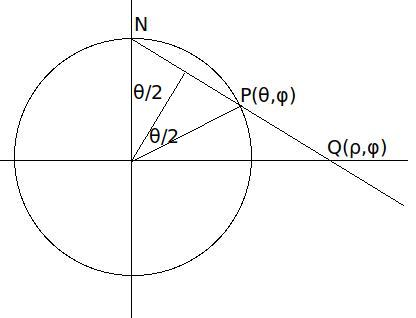
\includegraphics[scale=.60]{projecaoest1.jpeg}
 \caption{Projeção Estereográfica de um ponto, $(\theta,\varphi)$, 
 					da esfera, no plano, em um ponto, $(\rho,\varphi)$.}
 \label{projecao1}
\end{figure}

A partir da figura \ref{projecao1}, deve-se destacar o triângulo 
$\triangle ONQ$, veja a figura abaixo, onde é mostrado que o ângulo 
entre a reta traçada a partir do polo norte, N, até o plano xOy, 
e o eixo O$\rho$ é tal que seja igual à $\theta/2$, de modo que 
tenhamos a seguinte relação, $\rho = R\cot(\theta/2)$.

\begin{figure}[!ht]
 \centering
 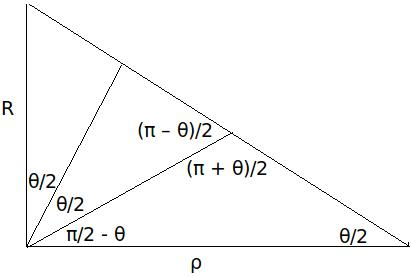
\includegraphics[scale=.5]{projecaoest2.jpeg}
 \caption{Ilustração que mostra a relação $\rho = R\cot(\theta/2)$.}
\end{figure}

Derivando a relação $\rho = R\cot(\theta/2)$, encontra-se,
%
\begin{align}
\nonumber d\rho &= - \frac{R}{2}\csc^2(\theta/2)d\theta \\ 
                &= - \frac{R}{2}(1 + \cot^2(\theta/2))d\theta,
\end{align}
%
De modo que tem-se a seguinte relação:
%
\begin{equation}
d\theta^2 = \frac{4R^2}{(R^2 + r^2)^2}d\rho^2,
\end{equation}
%
Tendo em conhecimento de que
%
\begin{equation}
\sin\theta = 2\sin(\theta/2)\cos(\theta/2),
\end{equation}
%
tem-se que:
%
\begin{equation}
\sin(\theta/2) = \frac{2\cot(\theta/2)}{1 + \cot^2(\theta/2)},
\end{equation}
%
Lembrando que $\rho = R\cot(\theta/2)$, tem-se o seguinte resultado:
%
\begin{equation}
\sin(\theta/2) = \frac{2R\rho}{R^2 + \rho^2},
\end{equation}
%
Inserindo os resultados encontrados para $d\theta^2$, $\sin^2(\theta/2)$, 
na na métrica da esfera, $ds^2 = R^2(d\theta^2 + \sin^2\theta d\varphi^2)$, 
encontra-se a seguinte relação para a métrica, no sistema de coordenadas 
da projeção estereográfica, $(\rho,\varphi)$:
%
\begin{align}
\nonumber ds^2 &= R^2(d\theta^2 + \sin^2\theta d\varphi^2) \\
               &= \frac{4R^4}{(R^2 + \rho^2)^2}(d\rho^2 + 
     \rho^2 d\varphi^2).
\end{align}
%
Lembrando que tem-se a seguinte relação, $\rho^2 = x^2 + y^2$, e de que, 
$x = \rho\cos\varphi$ e $y = \rho\sin\varphi$, vale a seguinte relação 
entre os sistemas de coordenada $(\rho,\varphi)$ e $(x,y)$:
%
\begin{equation}
dx^2 + dy^2 = d\rho^2 + \rho^2 d\varphi^2.
\end{equation}
%
Que nada mais é do que a transformação de coordenadas cartesianas para 
coordenadas polares. Dessa maneira tem-se que:
%
\begin{align}
\nonumber ds^2 &= R^2(d\theta^2 + \sin^2\theta d\varphi^2) 
\\ 
               &= \frac{4R^4}{(R^2 + \rho^2)^2}(dx^2 + dy^2)
\end{align}
%
De forma que, para encontrar a métrica da esfera, basta multiplicar 
a métrica do plano, $ds^2 = dx^2 + dy^2$, pela seguinte função:
%
\begin{equation}
f(\rho,R) = \frac{4R^4}{(R^2 + \rho^2)^2}.
\end{equation}

\section{Projetando o Polo Norte}


%%%%%%%%%%%%%%%%%%%%%%%%%%%%%%%%%%%%%%%%%%%%%%%%%%%%%%%%%%%%
\subsection{Introdução}

A projeção estereográfica é um mapeamento que projeta a 
esfera no plano, sendo definida em toda a esfera exceto 
em um ponto, neste caso escolheremos o 'polo norte'. Essa 
projeção é um funcional linear suave e bijetivo, é uma 
transformação conforme (preserva ângulos), mas não é uma 
isometria (não preserva distâncias nem áreas das figuras).

Seja a esfera $S_{\R}^2\subset\R^3 = \{(x,y,z)\in\R^3 \ 
| \ x^2 + y^2 + z^2 = R^2\}$, a projeção estereográfica é 
definida como o mapeamento no plano de um ponto $P(x,y,z)$
pertencente à esfera $S_{\R}^2$ em um ponto $P'(x',y')$ 
pertencente ao plano $\R^2$.

Em outras palavras projeta-se a esfera $S_{\R}^2$ através 
do 'polo norte' $N(0,0,R)$ no plano equatorial $z = 0$. 
A interseção de uma reta que liga o ponto $N$ e o plano
equatorial define um ponto $P'(x',y')$ no plano chamado 
de imagem estereográfica do ponto $P(x,y,z)$ definido 
pela interseção desta mesma reta com a esfera.


\begin{figure}[!h]
 \centering
 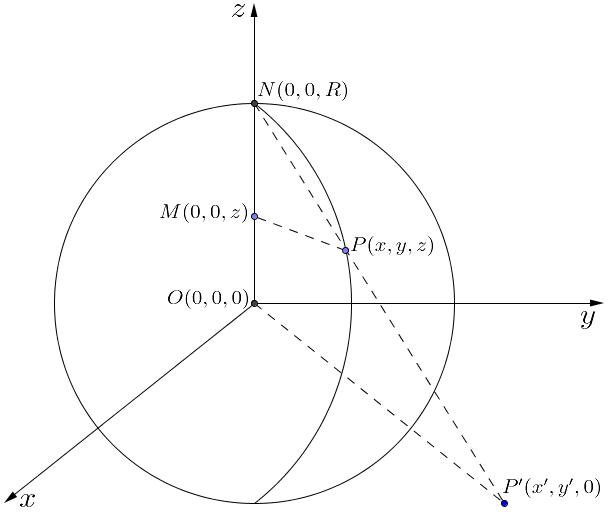
\includegraphics[scale=.6]{projecao1.JPG}
 \caption{Projeção Estereográfica da esfera no plano. 
 O ponto $P'(x',y')$ é a imagem
estereográfica do ponto $P(x,y,z)$.} 
\label{figura1}
\end{figure}



%%%%%%%%%%%%%%%%%%%%%%%%%%%%%%%%%%%%%%%%%%%%%%%%%%%%%%%%%%%%
\subsection{Coordenadas Cartesianas no Plano}

Analisando a figura anterior, temos dois triângulos 
retângulos semelhantes. Um deles é o triângulo $\Delta MNP$ 
e o outro é o triângulo $\Delta ONP'$:
%
\begin{equation}
\frac{\overline{MN}}{\overline{ON}} = 
\frac{\overline{MP}}{\overline{OP'}} 
\Rightarrow
\frac{z-R}{R} = \frac{\sqrt{x^2 + y^2}}
{\sqrt{{x'}^2 + {y'}^2}}
\end{equation}
%
Se fizermos $y = 0$ teremos também que $y' = 0$, pois 
movemos o ponto $P(x,y,z)$ para o plano $xOz$, mas os 
triângulos permanecem os mesmos. E se fizermos $x = 0$ 
teremos $x' = 0$ pois projetamos os triângulos para 
o plano $yOz$. Resolvendo individualmente as duas
condições encontramos que:
%
\begin{equation}
x' = \frac{Rx}{R - z} \qquad y' = \frac{Ry}{R - z}
\end{equation}
%
Elevando as duas relações encontradas para $x'$ e $y'$ 
ao quadrado temos que:
%
\begin{equation}
{x'}^2 + {y'}^2 = R^2\frac{(x^2 + y^2)}{(R-z)^2} 
= R^2\frac{(R^2 - z^2)}{(R-z)^2}
\end{equation}
%
Simplificando a relação acima temos que:
%
\[
{x'}^2 + {y'}^2  = R^2\frac{R + z}{R - z}
\]
%
Invertendo a transformação conforme, encontramos 
o seguinte resultado:
%
\[
\frac{z}{R} = \frac{{x'}^2 + {y'}^2 - R^2}
{{x'}^2 + {y'}^2 + R^2}
\]
%
Conhecendo este resultado podemos agora encontrar 
as relações para $x$ e $y$:
%
\begin{align}
x &= \left(1 - \frac{z}{R}\right)x' 
= \frac{2R^2x'}{{x'}^2 + {y'}^2 + R^2} 
\\
y &= \left(1 - \frac{z}{R}\right)y' 
= \frac{2R^2y'}{{x'}^2 + {y'}^2 + R^2}
\end{align}



%%%%%%%%%%%%%%%%%%%%%%%%%%%%%%%%%%%%%%%%%%%%%%%%%%%%%%%%%%%%
\subsection{Coordenadas Esféricas em Polares}

Agora iremos encontrar as coordenadas polares no 
plano $(\rho,\varphi')$ em função das coordenadas 
esféricas $(R,\theta,\varphi)$ e vice-versa. 
Utilizando a identidade $\rho = \sqrt{{x'}^2 + 
{y'}^2}$ e a relação para ${x'}^2 + {y'}^2$ deduzida 
anteriormente, temos que:
%
\[
{x'}^2 + {y'}^2 = \rho^2 = R^2
\frac{R + z}{R - z} \Rightarrow 
\rho = R\sqrt{\frac{R + z}{R - z}}
\]
%
Das coordenadas esféricas temos que $z = R\cos\theta$. 
Inserindo este resultado na equação anterior deduzida 
para $\rho$ chegamos ao seguinte resultado:
%
\[ 
\rho = \frac{R\sin\theta}{1 - \cos\theta}
\]
%
Lembrando das seguintes relações deduzidas na seção 
anterior:
%
\[ 
x' = \frac{Rx}{R - z} \qquad y' = \frac{Ry}{R - z}
\]
%
Podemos deduzir a relação para $\varphi$ em função das 
coordenadas esféricas:
%
\[
\tan\varphi' = \frac{y'}{x'} = \frac{y}{x} = 
\tan\varphi \Rightarrow \varphi' =
\varphi
\]
%
De modo que deduzimos as relações de transformação 
conforme entre as coordenadas esféricas e polares 
no plano.
%
\[
\left(\rho,\varphi'\right) 
\to \left(\frac{R\sin\theta}{1 - \cos\theta}, 
\varphi\right)
\]
%
Deduziremos agora as relações inversas $(R,\theta, 
\varphi)\to(\rho,\varphi)$. Temos que:
%
\[
\rho = \frac{R\sin\theta}{1 - \cos\theta} =
R\frac{2\sin(\theta/2)\cos(\theta/2)}
{2\sin^2(\theta/2)} = R\cot(\theta/2)
\]
%
Já foi mostrado que $\varphi' = \varphi$, então 
termina a demonstração da transformação inversa 
entre coordenadas esféricas e polares no plano:
%
\[
(\theta,\varphi) \to \left(\frac{1}{2} 
\cot^{-1}\left(\frac{\rho}{R}\right),\varphi'\right)
\]



%%%%%%%%%%%%%%%%%%%%%%%%%%%%%%%%%%%%%%%%%%%%%%%%%%%%%%%%%%%%
\subsection{Coordenadas Cilíndricas em Polares}

Nesta seção iremos encontrar a transformação de 
coordenadas cilíndricas $(r,\varphi,z)$ em coordenadas 
polares no plano $(\rho,\varphi')$. As coordenadas 
cilíndricas para as coordenadas dos pontos pertencentes 
à esfera são dadas por:
%
\begin{align}
r       &= \sqrt{x^2 + y^2}, 
\\
\varphi &= \tan^{-1}\left(\frac{y}{x}\right) 
\\
z'      &= z.
\end{align}
%
As coordenadas polares dos pontos pertencentes ao plano são:
%
\begin{align}
\rho     &= \sqrt{{x'}^2 + {y'}^2} 
\\ 
\varphi' &= \tan^{-1}\left(\frac{y}{x}\right).
\end{align}
%
Em coordenadas esféricas temos que $R = 
\sqrt{x^2 + y^2 + z^2}$. Comparando com as 
coordenadas cilíndricas:
%
\begin{equation}
(x, y, z) = (r\cos\varphi, r\sin\varphi, z), 
\end{equation}
%
tem-se que:
%
\begin{equation}
R^2 = r^2 + z^2 = \mbox{constante}.
\end{equation}
%
Em seções anteriores já foi demonstrado que:
%
\begin{equation}
x' = \frac{Rx}{R - z} \qquad , \qquad y' = \frac{Ry}{R - z}.
\end{equation}
%
De onde obtem-se imediatamente que:
%
\begin{equation}
\frac{y'}{x'} = \frac{y}{x} \Rightarrow \varphi = \varphi'.
\end{equation}
%
A seguinte relação também é imediata:
%
\begin{equation}
\rho^2 = {x'}^2 + {y'}^2 = \frac{R^2r^2}{(R - z)^2}, 
\end{equation}
%
que implica em:
%
\begin{equation}
\rho = \frac{Rr}{R -z}.
\end{equation}
%
Dessa maneira as relações de transformação das variáveis 
$(\rho,\varphi')$ nas variáveis $(r,\varphi,z)$ são 
as seguintes:
%
\begin{equation}
(\rho,\varphi') \to \left(\frac{Rr}{R - z},\varphi\right).
\end{equation}
%
Lembrando que $R(r,z) = \sqrt{r^2 + z^2}$ é uma função 
constante, dessa maneira é possível encontrar as relações 
inversas de transformação $(r,\varphi,z)\to(\rho,\varphi')$:
%
\begin{equation}
\rho = \frac{Rr}{R - z}, 
\end{equation}
%
implica que, 
%
\begin{equation}
z(\rho,\varphi') = \frac{\rho^2 - R^2}{\rho^2 + R^2}R.
\end{equation}
%
Utilizando-se do fato de que $r^2 = R^2 - z^2$ 
obtem-se que:
%
\begin{equation}
r(\rho,\varphi') = \frac{2R\rho}{\rho^2 + R^2}.
\end{equation}
%
Tem-se que as relações de transformação inversa são:
%
\begin{equation}
(r,\varphi,z) \to \left(\frac{2R\rho}{\rho^2 + R^2}, 
\varphi, \frac{\rho^2 - R^2}{\rho^2 + R^2}R\right).
\end{equation}
%


\begin{thebibliography}{}

\bibitem{Dubrovin}
Dubrovin, Fomenko, Novikov. Modern Geometry- Methods and Applications, 
Part 1, The Geometry of Surfaces, Transformation Groups and fields.

\end{thebibliography}
\include{3}

\printindex
\end{document}